% Preamble
\documentclass[16pt,a4paper]{article}
% or use the geomety package to change this
% default size is 10px
% {beamer} - for presentatins
% packages
% \usepackage[left=23mm, right=10mm, top=10mm, bottom=10mm]{geometry}
% \usepackage[margin=1.5cm]{geometry}

% for example lets create a remarkable size paper
\usepackage[paperwidth=15.6cm, paperheight=20.8cm, left=23.4mm, right=10mm, top=10mm, bottom=10mm, footskip=5mm]{geometry}
% \usepackage{amsmath, amsbsy} most used math package
% embed jpeg png
\usepackage{graphicx}
\usepackage[]{ulem}
% //this make all indents in the document 0
\setlength{\parindent}{0cm}
% this will make table of contents hypelinks and will allow to use hyperlinks in refs
\usepackage[]{hyperref}
    \hypersetup{hidelinks}

% User defined commands
% \newcommand{\commandname}[][]{definition}
\newcommand{\W}{\uwave{wavy lined text \\}}


\begin{document}
\pagebreak

\W
\W
\W

\title{A very nice sample title}
\date{April 30}
\author{Mariann Tapfer}
\maketitle
\tableofcontents
\section[The title in table of contents is different]{Introduction}
\subsection{Images}
This works with JPEG, PNG, EPS, PDF\\
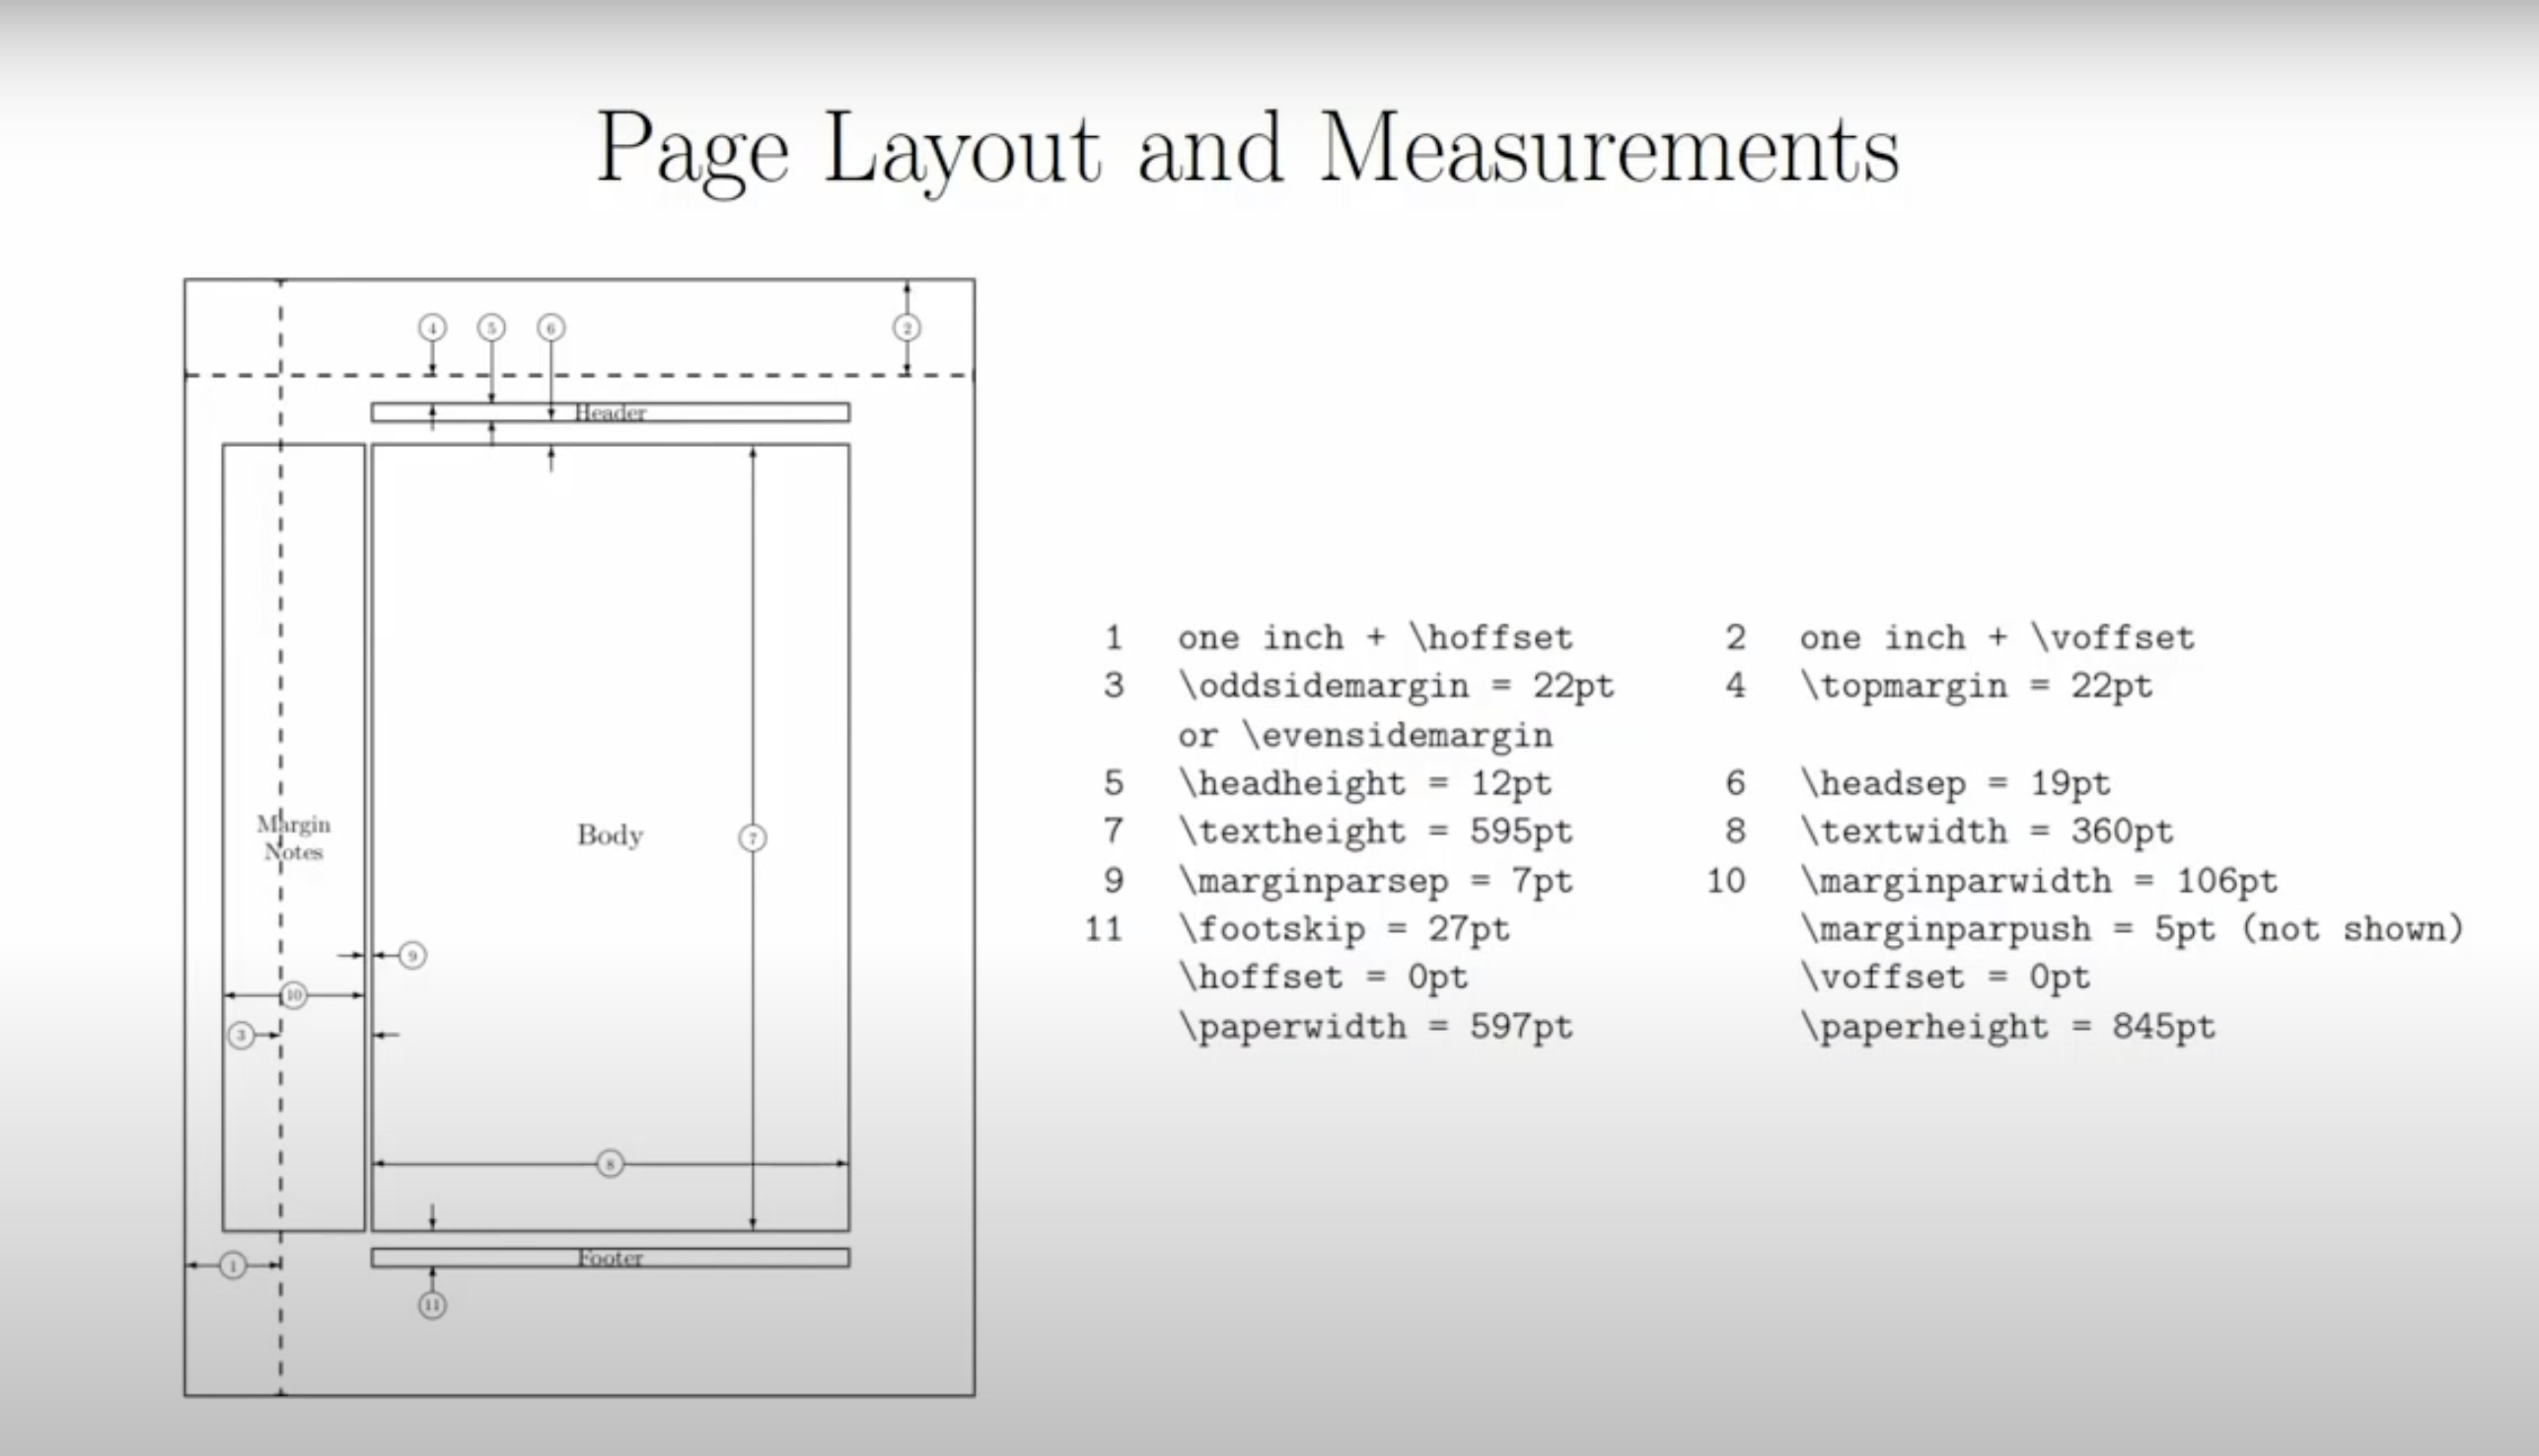
\includegraphics[width=10cm]{page_layput.png}\\
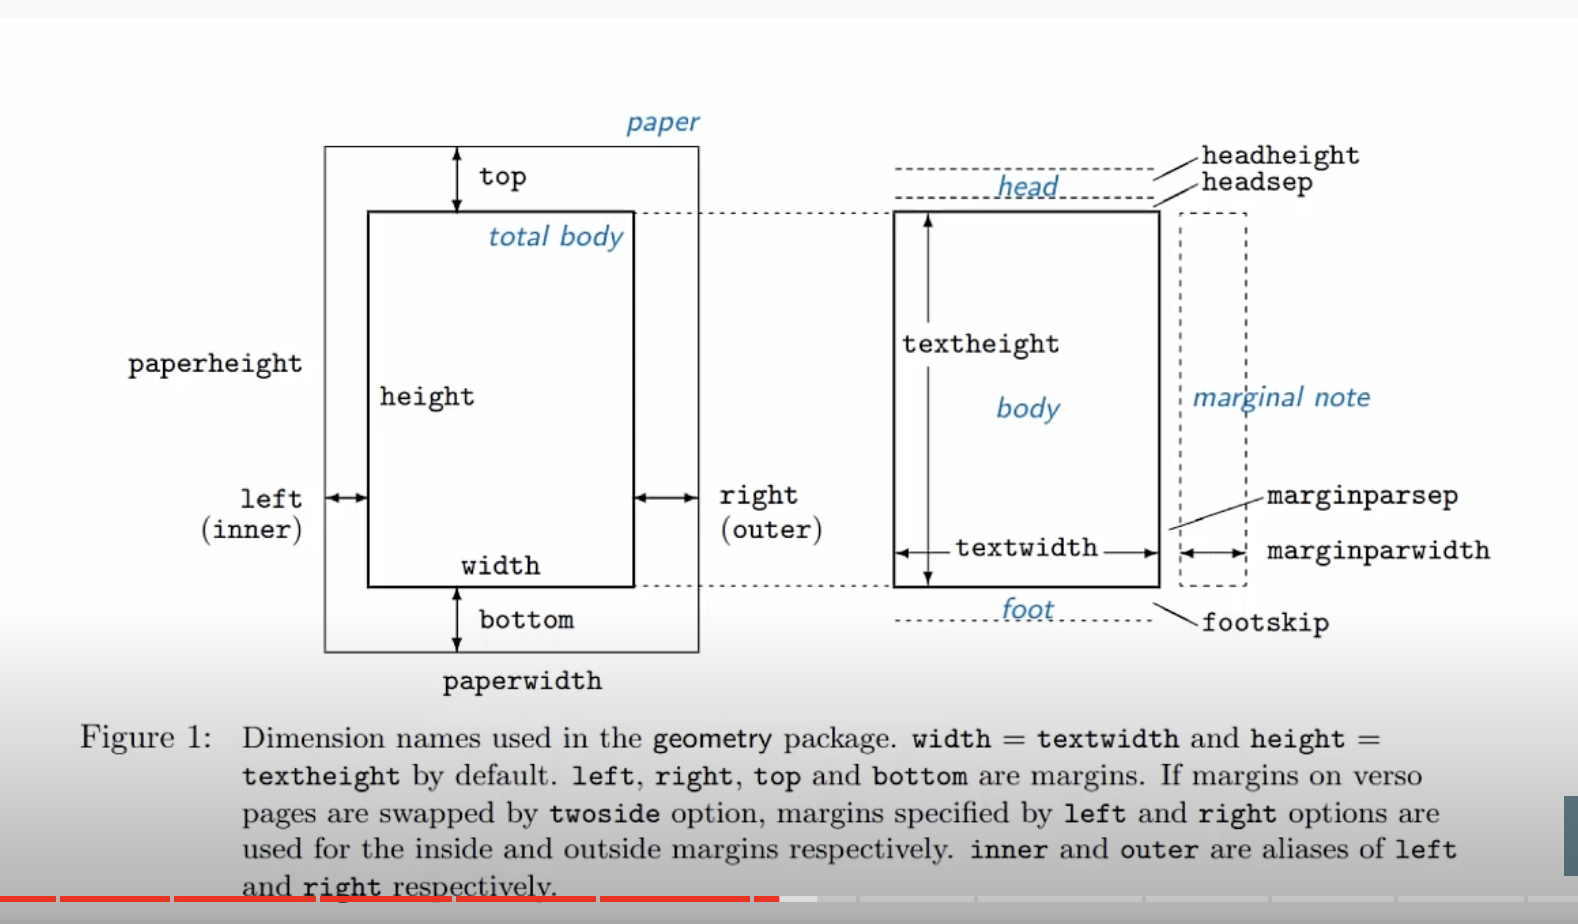
\includegraphics[scale=0.4]{margins.png}\\
\subsection{Table of contents}
For custom tables tocloft package might be useful.
\subsection{General} \label{sec:Mysec}
This is a sample introduction section.
This is the second linne in the section.
% \Large this will make all text after this large
{\Large this will make only the text inside the brakets large}
\textit{ this will make only the text inside the brakets italic}
\textbf{ this will make only the text inside the brakets bold}
\underline{this will make only the text inside the brakets underliend} \\
\textbf{\textit{\underline{ this will make only the text inside the brakets cold italic and underlined }}}
% this alters the intentation of the entire document by default there is new lines in intented
% \setlength{\parindent}{1cm}

\uline{Ulem pacage example. This is better for underline than regular underline, because it can break lines}

\uuline{and has more options}

\uwave{and has more options}



And this is the Third line. \\
This is how you change the line.

\section{Motivation}
The goal of this little document is to understand how to use latex and test it out a bit before starting to write my master thesis.

% \newpage
\pagebreak

\section{Commands}
\% is used for commenting out things in the .tex document.
\\ at the end of the line goes to new line. \\
Regular \emph{emphasized text}.
\textit{This will make only the \emph{text} inside the brakets italic}\\
\textrm{Roman text is default}\\
\textsf{Sans serif is also available}\\
\texttt{as is Typewriter – this could be used for code snippets for example}\\
By default text is fully justified and you need a much longer paragraph to really be able to see the effect here.
By default text is fully justified and you need a much longer paragraph to really be able to see the effect here.
By default text is fully justified and you need a much longer paragraph to really be able to see the effect here.
\begin{flushleft}
    This text is left aligned and you need a much longer paragraph to really be able to see the effect here.
    This text is left aligned and you need a much longer paragraph to really be able to see the effect here.
    This text is left aligned and you need a much longer paragraph to really be able to see the effect here.
\end{flushleft}
\begin{center}
    This text is centre aligned and you need a much longer paragraph to really be able to see the effect here.
    This text is centre aligned and you need a much longer paragraph to really be able to see the effect here.
    This text is centre aligned and you need a much longer paragraph to really be able to see the effect here.
\end{center}
\begin{flushright}
    This text is right aligned and you need a much longer paragraph to really be able to see the effect here.
    This text is right aligned and you need a much longer paragraph to really be able to see the effect here.
    This text is right aligned and you need a much longer paragraph to really be able to see the effect here.
\end{flushright}

Adding empty lines\\[\baselineskip]
Adding more than one empty line\\[2\baselineskip]
\section{Tables and arrays}
\subsection{Tables}
Table environment Tabular environment
this one has three columns aligned left, centre and right\\
\begin{tabular}{lcr}
    text    & text  & text \\
    l   & c & r
\end{tabular}\\
\begin{tabular}{|||l|c|r|}
    \hline
    text    & text  & text \\
    \hline
    \hline
    l   & c & r \\
    \hline
\end{tabular}\\
    "booktabs" package is most commonly used for making nicer tables, but also "tabularx", "colortbl" and "longtable"

\section{Lists}
\subsection{bullet}
\begin{itemize}
    \item [$\rightarrow$] First item
    \item Second item
    \item [just random text] Second item
    \item Second item
    \item [] Third item
    \begin{itemize}
        \item sub item
        \item another sub
    \end{itemize}
\end{itemize}
\subsection{numbered list}
\begin{enumerate}
    \item Apple
    \begin{enumerate}
        \item Granny Smith
        \item Valge klaar
    \end{enumerate}
    \item Banana
    \item Pear
\end{enumerate}

\section{Random}
\subsection{Non breakable space}

Non breakable space looks like this~and this space will not be broken appart by~line (example here) changes
\subsection{Space}
This text is centre \hspace{10mm} aligned and you need a much longer paragraph to really be able to see the effect here.
This text is centre aligned and you need a much longer paragraph to really be able to see the effect here.\vspace{2cm}
This text is centre aligned and you need a much longer paragraph to really be able to see the effect here.
\subsection{Boxes}

\fbox{text is centre aligned and you need a much longer paragraph to really be able to see the effect here.}
\subsection{Line and dot fill space}
text is centre aligned and you \hrulefill\\need a much longer paragraph to really \dotfill 34\\be able to see the effect here.\\
\rule{\linewidth}{1mm}
\begin{center}
    \rule{3cm}{2mm}
\end{center}

\section{References and citations}
\cite{sane_brief_2021}
Some more text in this paragraph to test if intelligense works. \cite{}
\bibliography{source.bib}
\bibliographystyle{plain}


\end{document}